\documentclass{article}
\usepackage[utf8]{inputenc}
\usepackage[margin=1in,left=1.5in,includefoot]{geometry}
\usepackage{booktabs}
\usepackage{graphicx}
\usepackage{hyperref}
\usepackage{wrapfig}
\usepackage{amsmath}
\usepackage{amssymb}
\usepackage[galician]{babel}

% Header & Footer Stuff

\usepackage{fancyhdr}
\pagestyle{fancy}
\lhead{Visión por Computador Aplicada}
\rhead{614G030332425}
% \fancyfoot{}
% \lfoot{Pablo Chantada Saborido \& José Romero Conde}
% \fancyfoot[R]{}

% The Main Document
\begin{document}
	\begin{center}
		\LARGE\bfseries PRÁCTICA II\\
		\small Pablo Chantada Saborido \& José Romero Conde
		\line(1,0){430}
	\end{center}
	
\vspace*{380pt}
	
\begin{figure}[h]
	\centering
	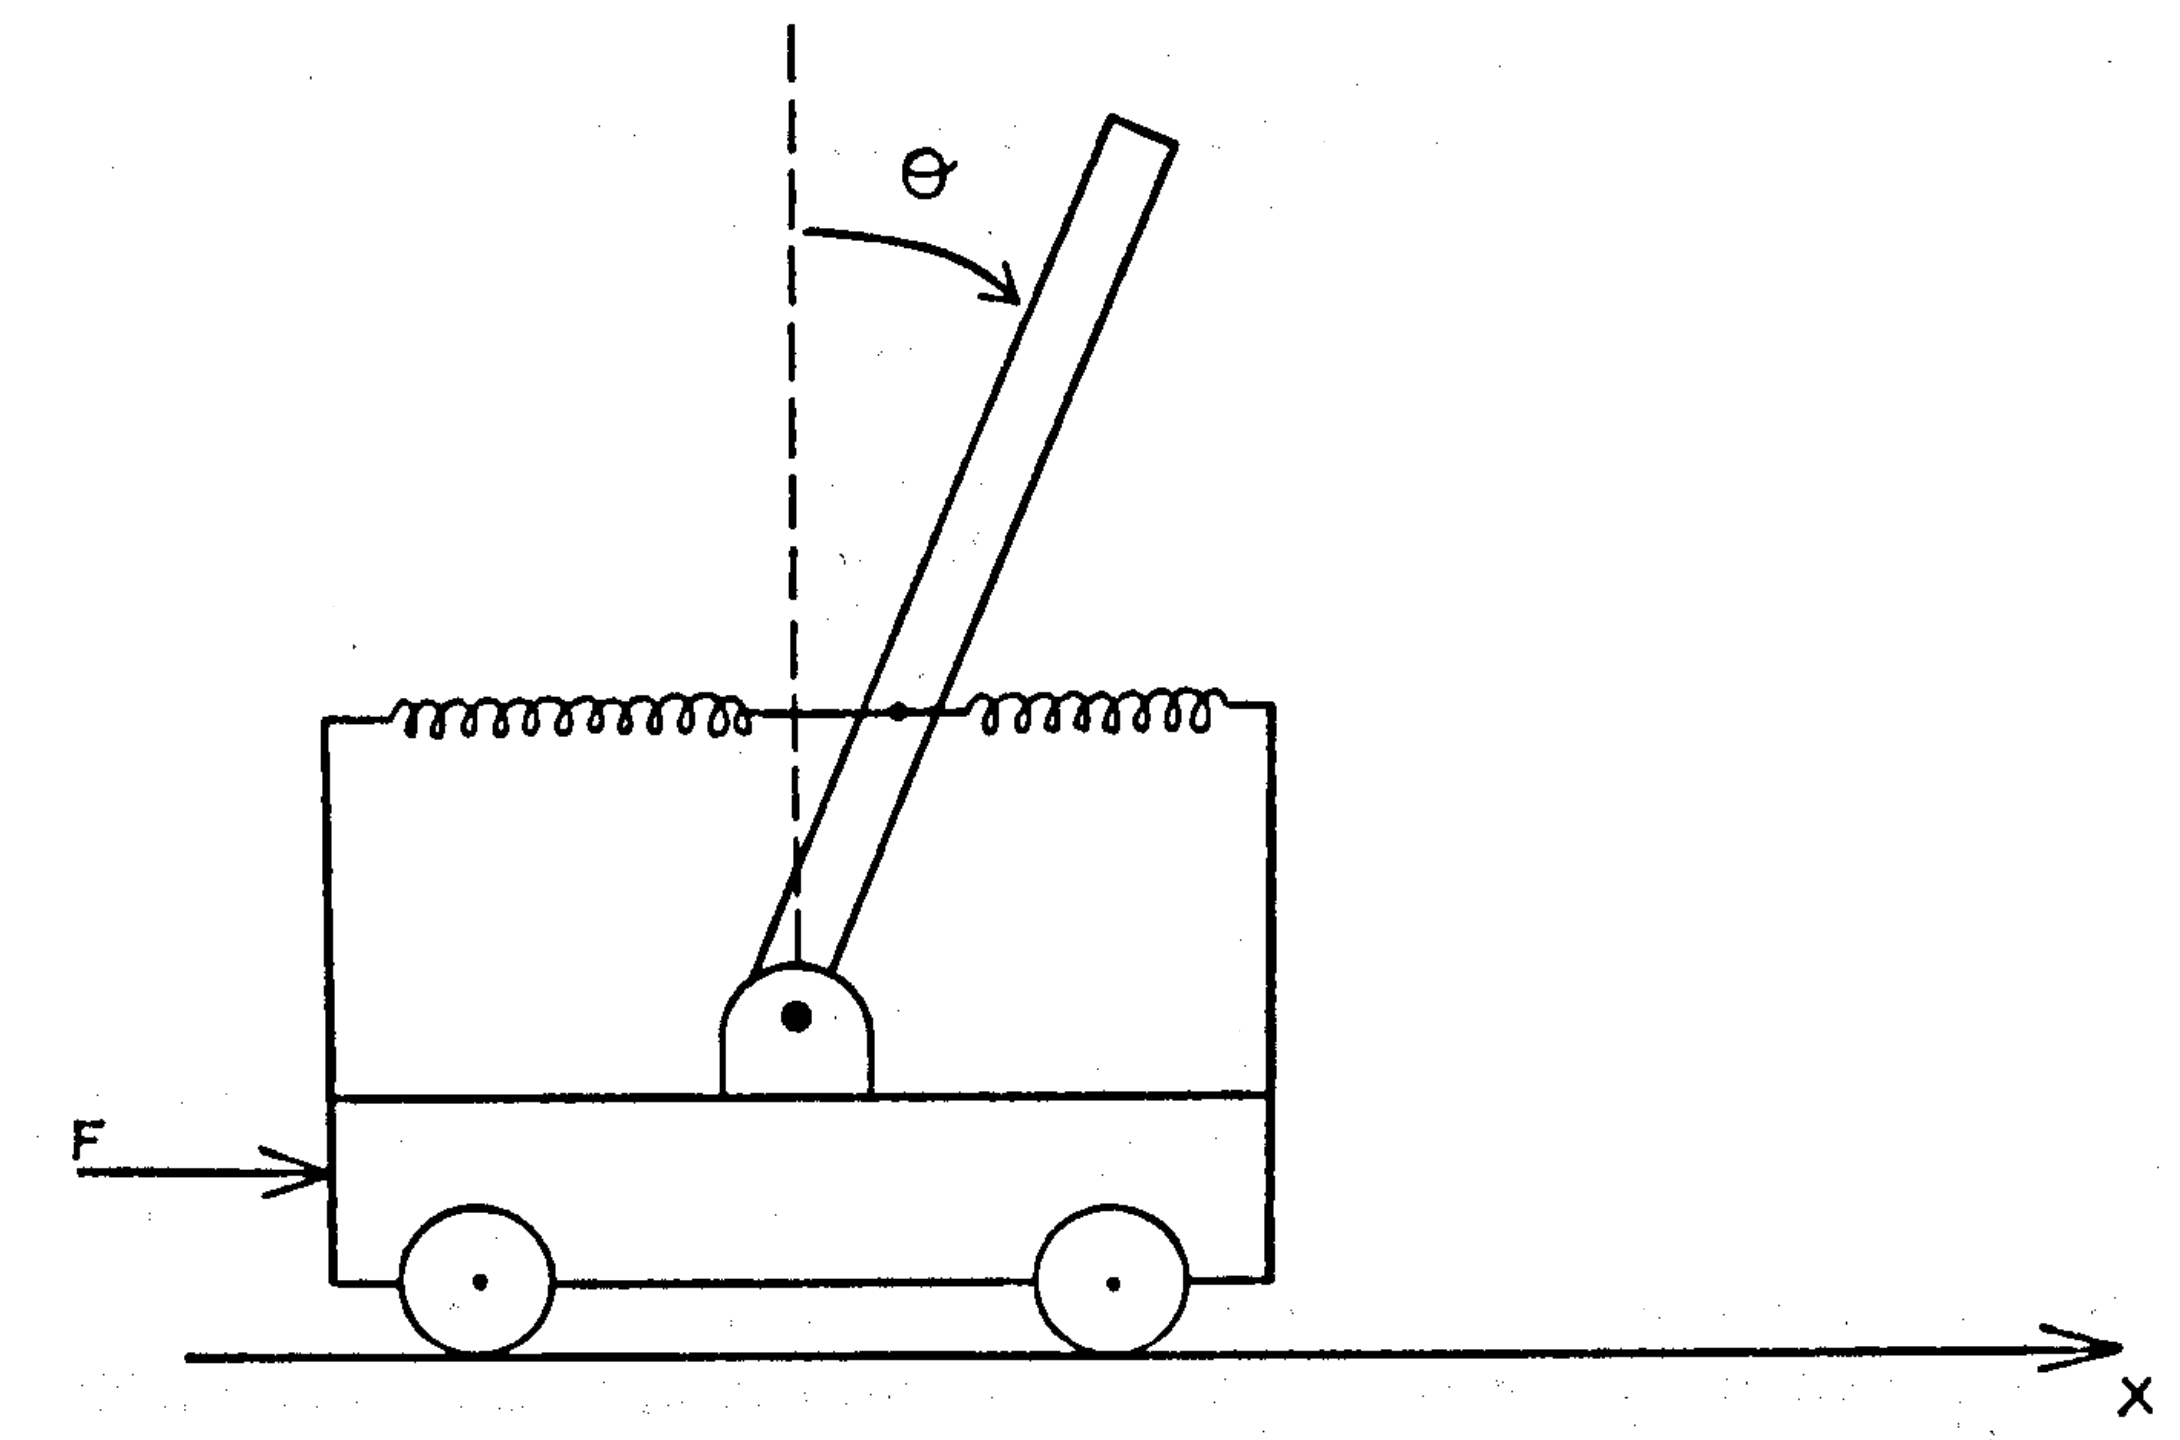
\includegraphics[width=0.7\linewidth]{portada}
	\label{fig:portada}
\end{figure}
	
\thispagestyle{empty}
	
\newpage

\tableofcontents

\newpage
	
	
\section{Introdución}
\subsection{O problema}

Despois de ler e comprender o enunciado da práctica, e de examinar as imaxes unha por unha, chegamos ás seguientes observacións:
\begin{itemize}
	\item Entre as imaxes de barcos existe unha gran variación de pose, escala, condicións de iluminación, proporción que ocupa na escena real (en metros) e proporción que ocupa na imaxen (píxeles). Ademáis os elementos en sí (barcos e peiraos) presentantan moita variación interclase (aínda que os barcos sexan todos industrais son distintos entre eles, e os peiraos poden estar baleiros ou cheos de montañas de area) e incluso unha maior similitude intraclase (sobretodo no caso barco-atracado contra barco-non-atracado).
	\item O alcance da práctica de esta asignatura era suficientemente limitado como para resolver o problema dun xeito satisfactorio. Creemos que poderíamos entrenar unha Rede de Neuronas Artificiais para resolver un subproblema o un problema maior con fin de que a Rede principal o teña máis doado para aprender. No obstante non é o que se pide entón aínda que preferiríamos resolver o problema dunha forma \emph{maís científica} por cuestións de tempo e alcance non o fixemos.
	\item En calqueira escenario (sexa unha práctica con fins docentes ou un traballo no mundo real) existe un problema co cómputo, no noso caso porque disponemos de poucos recursos para adestrar a Rede e no caso real porque o cálculo é posible que precise ser ou a tempo real ou nun sistema embebido, en calqueira caso recursos límitados. 
\end{itemize}

Estas observacións dirixiron o noso \emph{modus operandi}.

\subsection{O noso \emph{modus operandi}}

Aínda que teñamos cursadas asignaturas de aprendizaxe non somos, en nigún caso, expertos no adestramento de Redes de Neuronas Artificiais. Por esta razón preferimos ser cautos e explorar maitas opcións, todas as que podamos, aínda que o noso coñecemento pode (e debería) guiar esta búsqueda, tomamos a decisión de non tomar poucas decisións ó principio, e que fora a evidencia a que avale as conclusións. Por esto en vez de faceren unha Red estática, a fixemos altamente flexible. Referímonos a que fixemos un \emph{script} que recibe como argumento unha gran cantidade de hiperparámentros, de xeito que sexa maís cómodo probar. Despóis de algunhas probas (e acompañadas de lecturas da literatura) chegamos ó noso \emph{baseline}.

\section{Clasificación Ship/No-ship}
\subsection{Modelo base}

Describimos agora o noso modelo \emph{baseline}, que valeunos para iterar y comparar resultados. O modelo componse dos seguientes elementos:

\begin{itemize}
	\item  \textbf{EfficientNet.} \cite{tan2019efficientnet} Usámola como CNN (\emph{Convolutional Neural Network}) de partida. Orixinalmente pensamos que tiña como requirimiento que as imaxes sexan de tamaño $(244,244,3)$. E como as imaxes son (i) rectangulares (ii) de distinto tamaño entre sí; tivemos que implementar un recortador automático de \emph{o cadrado máis grande} que chamamos desde os \texttt{DataLoader} de adestramento e proba. Máis tarde decatámosnos que a Rede era realmente capaz de procesar imaxes de calqueira tamaño porque ten ó final un \texttt{Global Pooling}. No obstante, como de calqueira xeito os \emph{mini-batches} tiñan que ser todos del mismo tamaño (paralelepípedos) decidimos quedarnos ca idea de recortalas imaxes da forma mencionada. \\

Máis tarde, non obstante probamos con outros tamaños para o parelelepípedo, coa esperanza de que imaxes rectangulares ofrezcan mellores resultados (en vez de as cadradas) porque estas teñen máis información. Para a nosa sorpresa a evidencia demostrou moito mellor rendimento con imaxes cadradas. Hipotizamos que débese a que como da mesma imaxe rectangular, os cadrados resultantes do resultado aleatorio son realmente distintos entre sí, recortar rectangulos en cadrados pode supor un bo aumento de datos implícito. \\

En xeral a motivación para escaller esta rede e non outra débese á terceira observacións da sección 1.1 e á forma que tiveron os autores da Rede de atacar este problema directamente. Con respecto a que EfficientNet en contreto usamos: despóis de probar ca EfficientNetB3 e observar malos resultados decidimos mudar á EfficientNetB4 e nos quedamos nesta e non subimos á EfficientNetB$i \; | i\; \in \{5,6,7\}$ precisamente por limitacións de cómputo.

	\item \textbf{Aumento de datos.} O aumento de datos nesta fase esencialmente consta de dúas partes, por un lado, as transformacións de \texttt{torchvision.transforms} e por otro imaxes recortadas a man. Con respecto ó  primeiro, nosotros usamos: volteos horizontais, fluctuacións leves na cor, tamén leves transformacións afíns e conversión a blanco e negro con baixa probabilidade. O segundo punto é que recortamos manualmente as imaxes de barcos de forma que queden centrados e sen fondo que estorbe, engadíronse estas imaxes ó conxunto de datos cando especificabase aumento de datos. Desta forma conseguimos dúas cousas distintas: 
	\begin{itemize}
		\item Representar máis variacións que as presentes no conjunto de adestramento, ca esperanza de que se sí ocurriesen no conxunto de proba, estaríamos preparados. Por exemplo, como observamos imaxes de noite ou con chuvia encontramos razonable incluir a conversión a blanco e negro.
		\item Representar con menos ruído adicional o que sí queremos aprender. Porque aínda que é beneficioso para a Rede someterse a moita variación, tamén dificulta o adestramento (é un problema máis difícil).
\end{itemize}

Sobre o aumento de datos comentar que a relación dos hiperparámetros que o definen e problemática para nos faceren probas: se cambiamos varios de unha vez non está necesariamente claro a cal dos cambiados débese a mellora ou empeora do rendimiento; se, en cambio, cambiamos só un de cada vez, a búsqueda no espacio de hiperparámetros do aumento de datos vólvese prohibitiva. E por isto que sabemos que a nosa configuración debe ser subóptima, pero non temos nada para evitalo.
\item Un \textbf{MLP} (Perceptrón Multicapa ou \emph{Multi-layer Perceptron} en ingés) de tres capas, sobre a saída da Rede. A saída da última capa \texttt{nn.Softmax()} ten 2 o 3 neuronas según se quería clasificar en \{no barco, barco\} o en \{no barco, barco no amarrado, barco amarrado\}. Tamén probamos con un perceptrón simple (unha capa) pero a evidencia demostrou que os resultados eran mellores con tres. Como o número de neuronas na primeira capa (a saída da CNN) era máis grande ca o número de exemplos, a rede podería ter aprendido unha solución trivial co conxunto de adestramento e non xeneralizar en absoluto. Por esto mismo decantamos por usar a ben coñecida técnica de regularización \emph{DropOut} \cite{srivastava2014dropout}. 
\end{itemize}

\subsection{Adestramento e evaluación}

O adestramento foi díficil e ademáis somos inexpertos porén indentificamos algúns problemas para os que atopamos solución. Aquí preséntanse:
\begin{itemize}
	\item \textbf{Datos non balanceados.} Observamos que a Rede, \emph{hackeando} as nosas métricas decidía que todas as imaxes eran barcos. Esto débese ó desbalanceo dos datos (147 contra 88) dónde unha solución tan trivial e erronea como solo predecir unha clase non estaba tan penalizado con metricas como a precisión. Afrontamos isto alterando a probabilidade de ocurrencia das clases de forma que se antes, ó escolleren unha imaxe de \texttt{DataLoader}, $p(X=barco) = \frac{147}{147+88}$ ahora $p(X = barco) = 0.5$. Para ello usamos a utilidad \texttt{WeightedRandomSampler} de torch.
	\item \textbf{Similitud nos datos.} Non creemos conveniente que a Rede esté totalmente segura de que un barco non está (porque igual é pequeno ou está ocluído) cando ela dí que non hai barco na imaxe. Por isto, e para que xeneralice millor adoptamos a idea de \cite{DBLP:journals/corr/SzegedyVISW15} donde as etiquetas en vez de ser [0, 1] para non-barco e [1, 0] para barco, son [$\epsilon$,$1 - \epsilon$] e [$1- \epsilon$,$\epsilon$] respectivamente, onde fixamos $\epsilon = 0.1$.
	\item \textbf{Capacidade do modelo.} Orixinalmente usamos a EfficientNetB0, pero apreciando malos resultados decidimos mudar á EfficientNetB3 e logo á EfficientNetB4, que é un pouco máis grande pero precisamente como narran no artículo, é eficiente. Probamos con outras alternativas como as clásicas ResNet e VGGNet sen conseguiren melloras nos resultados que pagasen a pena a diferencia no consumo de recursos.
	\item \textbf{Mínimos locais.} Para aliviar as consecuencias da dificultade do adestramento implementamos un \texttt{learning\_rate} que, con unha certa paciencia, mediaba a sua valor. \footnote{Esta paciencia mencionada e a do \emph{earlystopping} poden ambas ser axustadas como \emph{flags} no noso \emph{script}.}
	\item \textbf{Sobreajuste y xeneralización.} Para cercionarnos de que a Rede aprendía correctamente, añadimos una penalización de la norma euclídea dos parámetros na función de perdida, es decir, regularización Tikhonov. Atopar valores axeitados para $\lambda$ foi especialmente difícil.
\end{itemize}


\begin{wrapfigure}{l}{0.3\textwidth}
	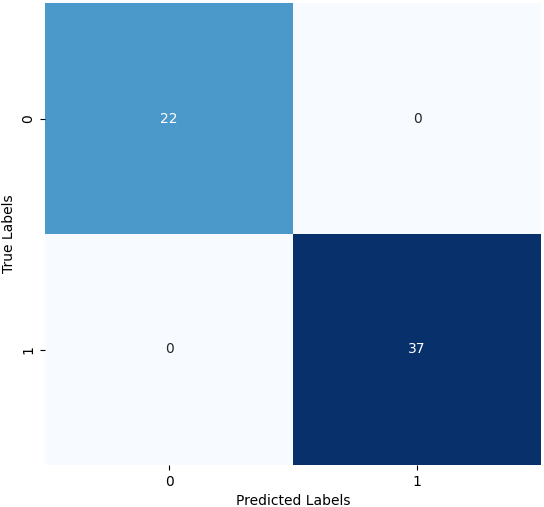
\includegraphics[width=1\linewidth]{cmEj1} 
	\label{fig:cmEj1}
	%\caption{Matriz de confusión para el primer ejercicio}
\end{wrapfigure}


Outras consideracións sobre o adestramento que consideramos menos profundas y más ordinarias son: como optimizador hemos usado AdamW\cite{DBLP:journals/corr/abs-1711-05101} con un \texttt{learning\_rate} de $10^{-3}$ ou $10^{-4}$. Usamos un \texttt{batch\_size} de 16, que aunque es relativamente pequeño, no mucho más pueden hacer nuestros portátiles. Por fortuna un de nos dispoñía a tiempo parcial de unha NVIDIA 4070 cedida pola Universidade e nela podíamos usar ata 64 imaxes á vez. Aínda así o tempo máquina reconocemos foi un cuello de botella. 

Con respecto ós resultados obtidos nesta primeira iteración, poden observarse a grandes rasgos na matriz de confusión da esquerda, a cal nosotros prudentemente podemos dicir que estamos orgullosos porque as predicciones da Rede concentranse nas etiquetas verdaderas, errando soamente [DEPENDE DE LA IMAGEN USADA]. Figuras de las curvas de pérdida y precisión en aprendizaje o de las etiquetas predichas por la red para algunas imágenes en concreto pueden encontrarse para este ejercicio y el siguente en el Apéndice al final del documento.


\section{Clasificación Docked/Undocked}

Nós concebimos este exercicio como unha extensión do anterior, deste xeito pensamos en reutilizar todas as representacións aprendidas.
\begin{itemize}
	\item Cuando especifícase \texttt{pretrained=True}, a nosa Rede non toma os parámetros de Imagenet, senon do exercicio anterior. Deste xeito xa ten moito aprendido e o proceso de optimización será más doado.
	\item Como agora a cabeza da Rede tee 3 neuronas pero antes tiña 2, en vez de inicializar aleatoriamente las tres neuronas, dous copianse e só unha inicializase aleatoriamente. De novo, deste xeito ten menos traballo por diante.
\end{itemize}

\subsection{Resultados}

\begin{wrapfigure}{l}{0.3\textwidth}
	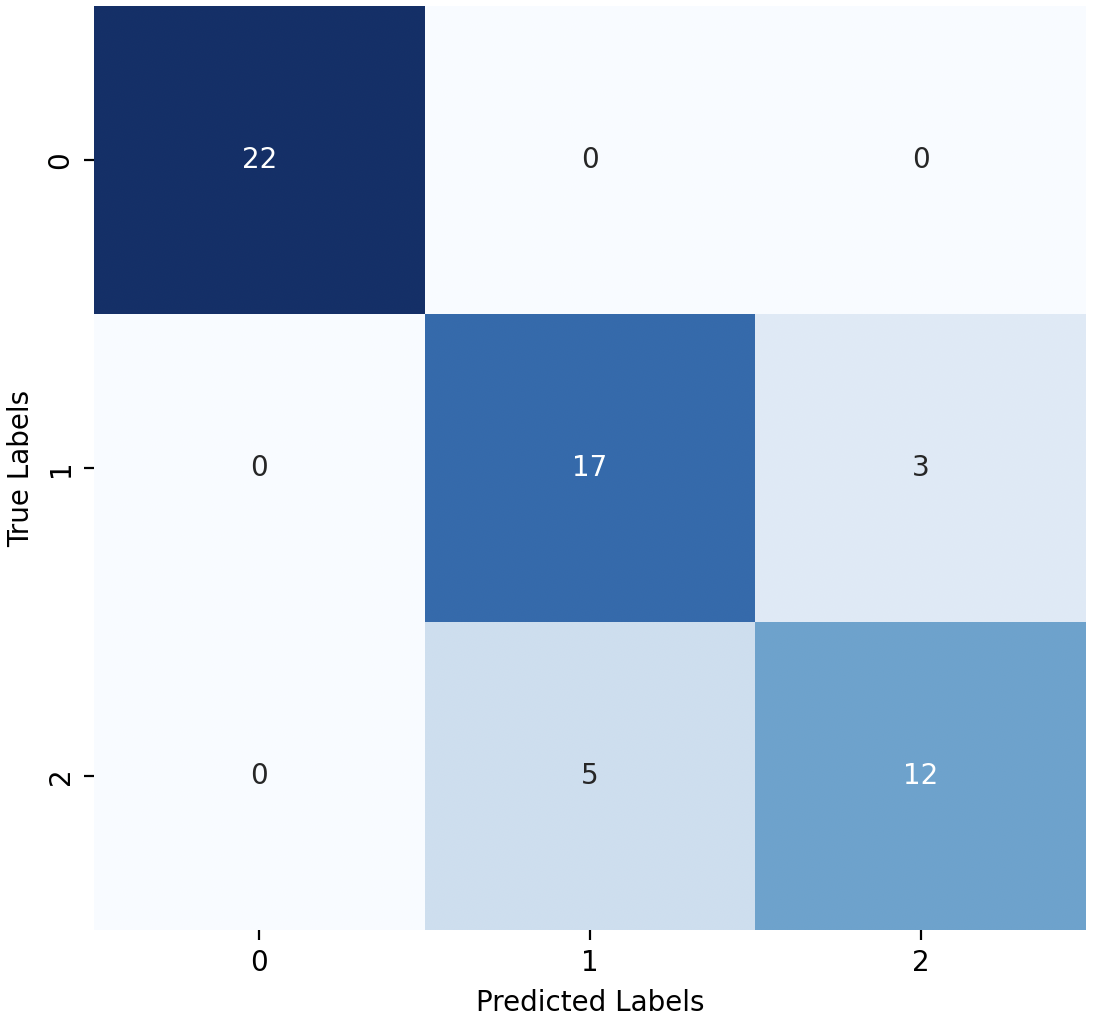
\includegraphics[width=1\linewidth]{cmEj2} 
	\label{fig:cmEj2}
	%\caption{Matriz de confusión para el segundo ejercicio}
\end{wrapfigure}

Ainda que a priori semella que son peores resultados que no exercicio 1, queremos señalar las siguientes observaciones:

\begin{itemize}
	\item Agora o problema orixinal (barco contra no barco) está totalmente resolto (no barco tiene la etiqueta de 0). A isto encontramoslle a seguiente intuición: que a Rede se esforce nun problema máis complexo fai que sexa máis capaz de resolver o problema sinxelo.
	\item As diferenzas entre as clases atracado contra no atracado son realmente sutiles [FOTO] e a un humano (nós probamos con amigos) que non foi \emph{adestrado} cas etiquetas tamén pode resultarlle complexo resolver. 
	\item Non obstante en xeneral poderíamos dicir que malia non seren a clasificación perfecta, polo  menos é bastante diagonal.
\end{itemize}

\section{Evaluación dos modelos}

Na tabla a continuación mostránse os resultados da precisión das prediccións da Rede cos datos de proba, a separación de datos adestramento e proba foi dun 80\%

\begin{table}[h]
\begin{tabular}{l|ll|rl|}
\cline{2-5}
                               & \multicolumn{2}{l|}{Non preentrenado}                        & \multicolumn{2}{r|}{Preentrenado}                            \\ \cline{2-5} 
                               & \multicolumn{1}{l|}{Non aumento de datos} & Aumento de datos & \multicolumn{1}{r|}{Non aumento de datos} & Aumento de datos \\ \hline
\multicolumn{1}{|l|}{2 clases} & \multicolumn{1}{l|}{}                     &                  & \multicolumn{1}{r|}{}                     &                  \\ \hline
\multicolumn{1}{|l|}{3 clases} & \multicolumn{1}{l|}{}                     &                  & \multicolumn{1}{r|}{}                     &                  \\ \hline
\end{tabular}
\end{table}


\section{Conclusión}

Agradecemos que o conxunto de datos desta práctica fora realista porque intentando obter mellores resultados tivemos que probar e aprender moitas cousas. Creemos, non obstante, que se tivesemos que resolver este problema nun contexto real, debería intentarse algunha aproximación más centrada en visión e non tan \emph{darlle os datos á rede e que ela aprenda}. Ou incluso usar arquitecturas máis sofisticadas que intenten resolver un problema más complexo como segmentación coa esperanza de que o rendimento na tarea más sinxela de clasificación véxase mellorado.

\section{Apéndice}

\begin{figure}[h]
	\centering
	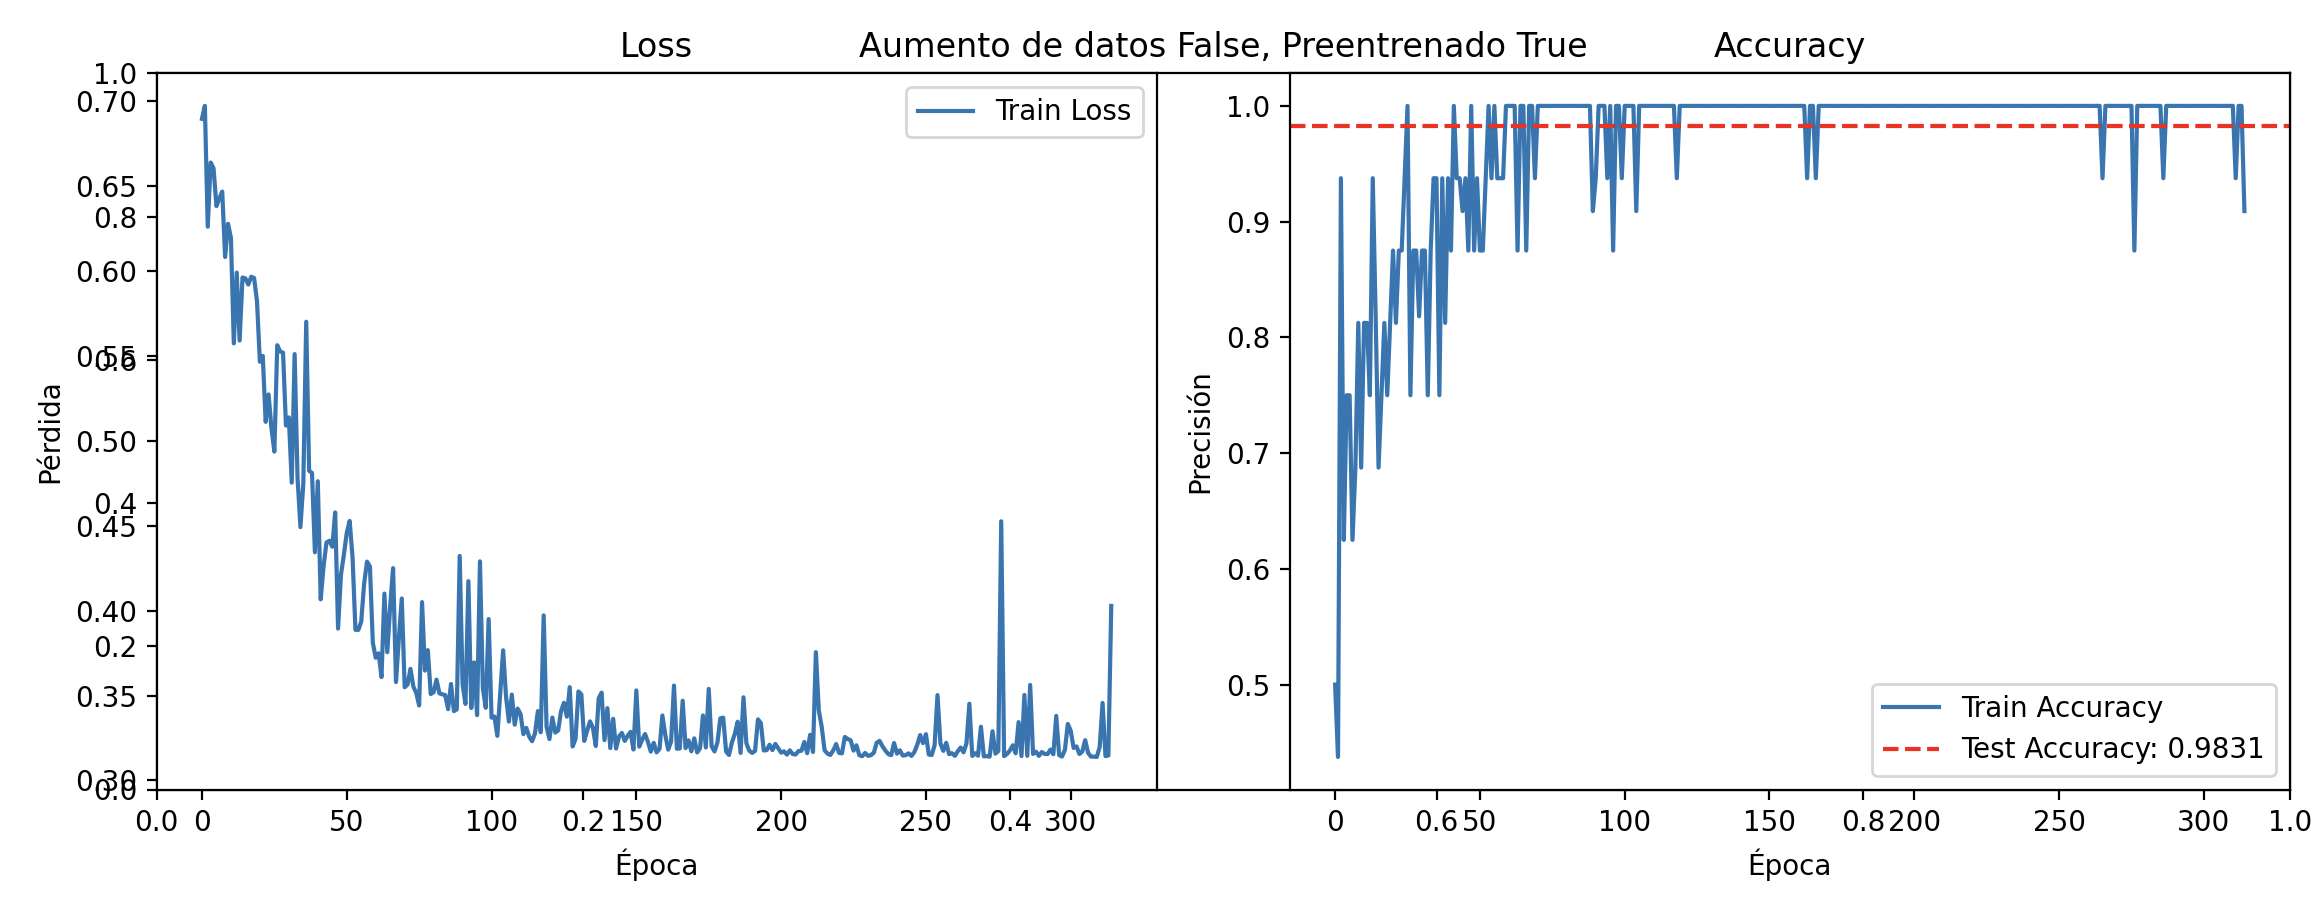
\includegraphics[width=0.9\linewidth]{lossEj1}
	\label{fig:lossEj1}
	\caption{Loss y Accuracy para el primer ejercicio}
\end{figure}

\begin{figure}[h]
	\centering
	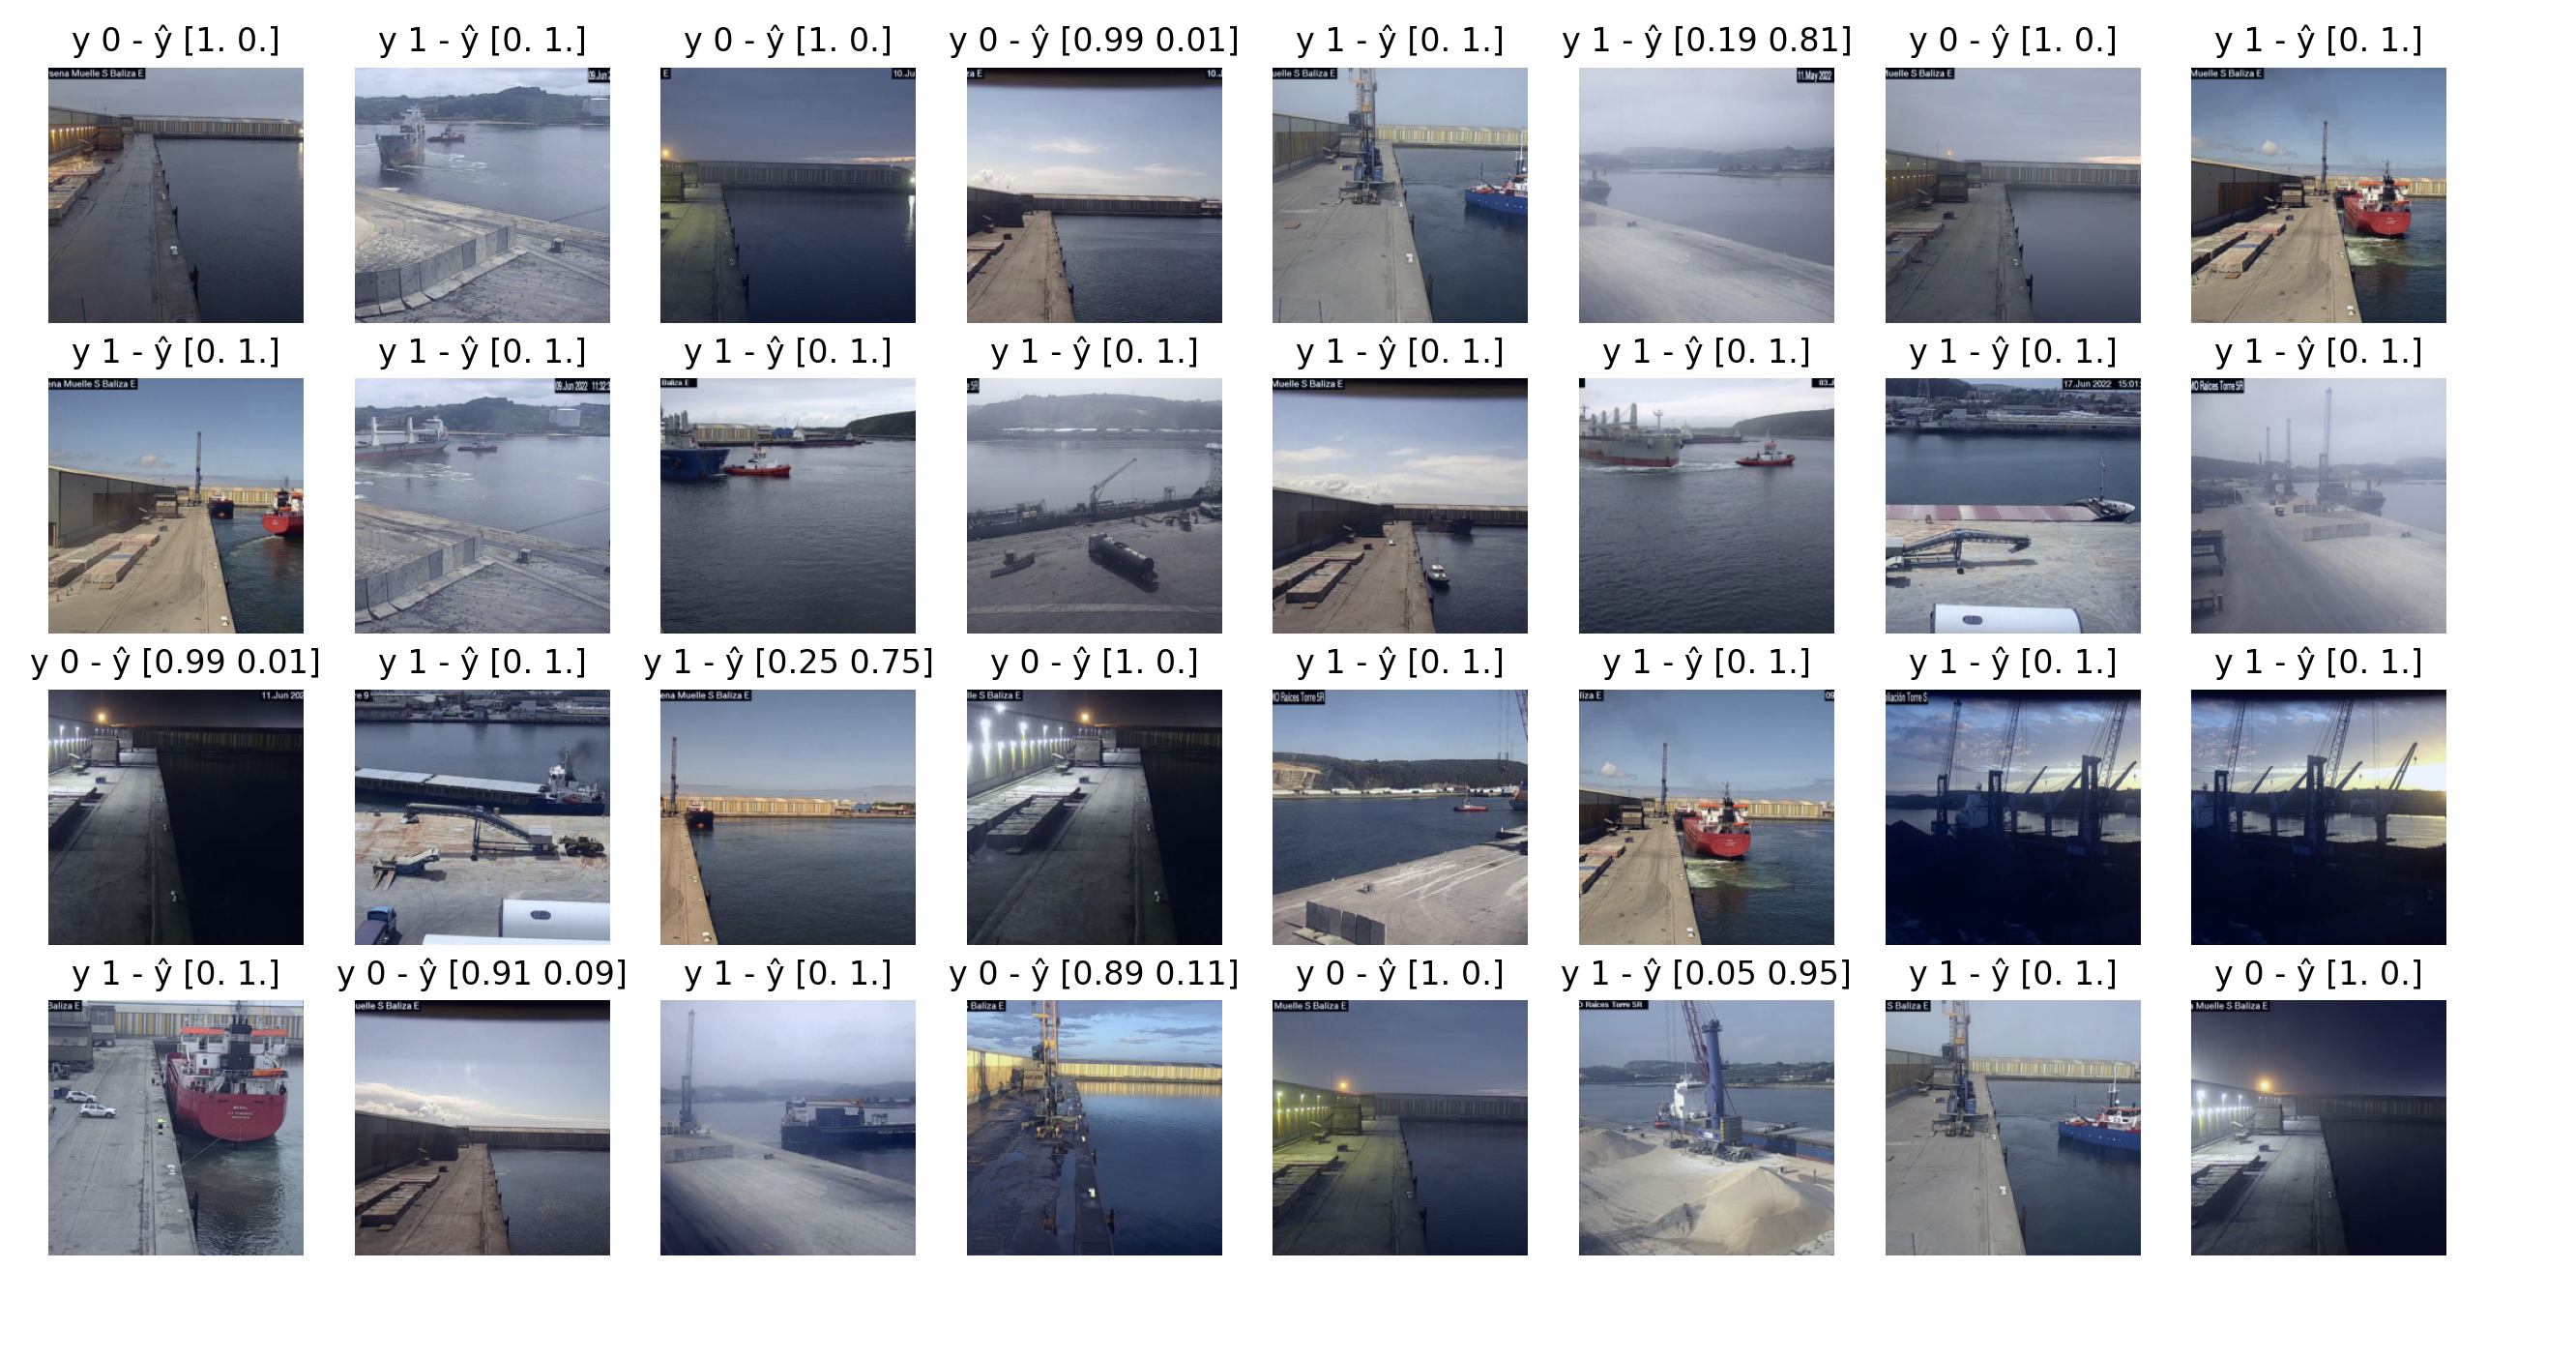
\includegraphics[width=0.8\linewidth]{imagenesEj1}
	\label{fig:imagenesEj1}
	\caption{Imágenes con su etiqueta correcta y el vector SoftMax predicha por la red para el primer ejercicio}
\end{figure}

%\begin{figure}[h]
%	\centering
%	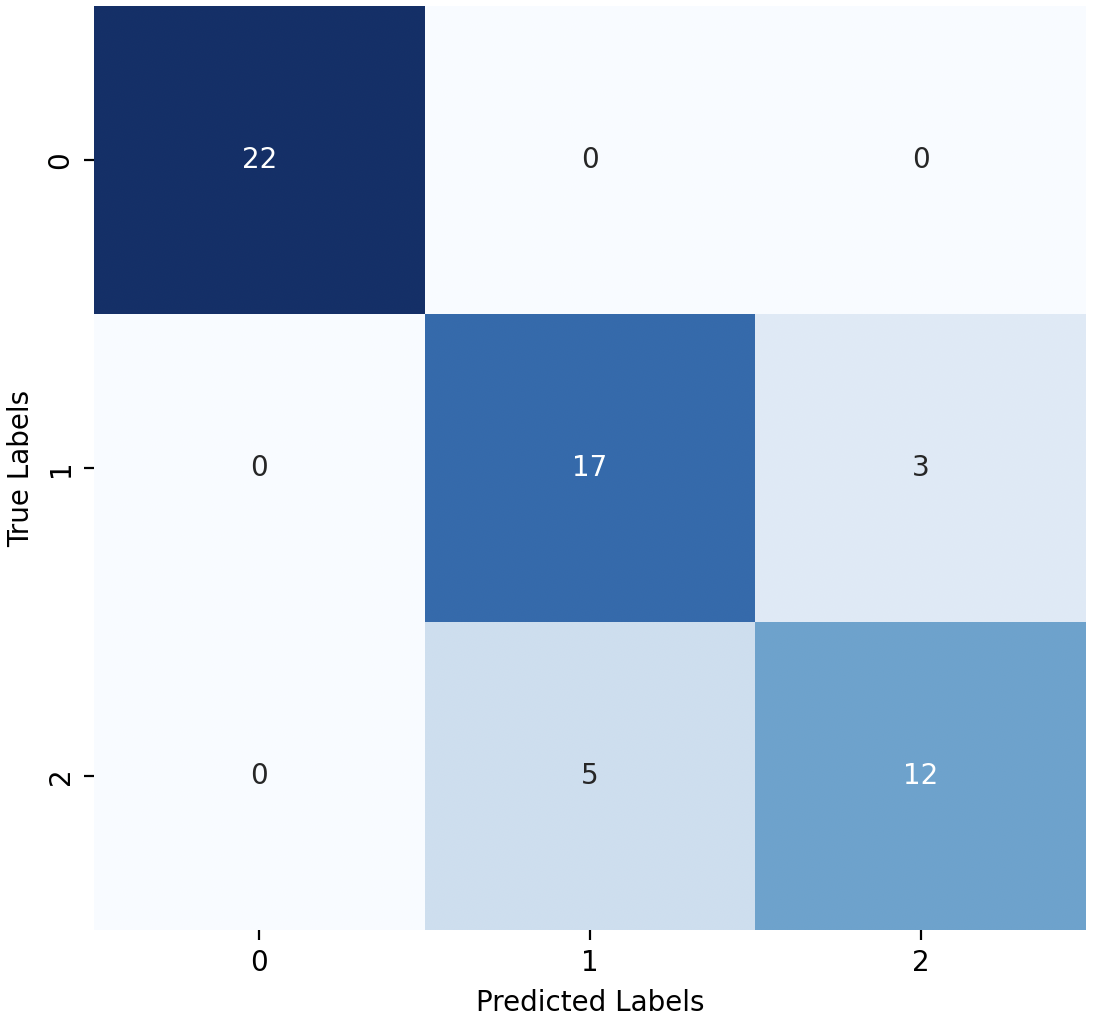
\includegraphics[width=0.5\linewidth]{cmEj2}
%	\label{fig:cmEj2}
%	\caption{Matriz de confusión para el segundo ejercicio}
%\end{figure}

\begin{figure}[h]
	\centering
	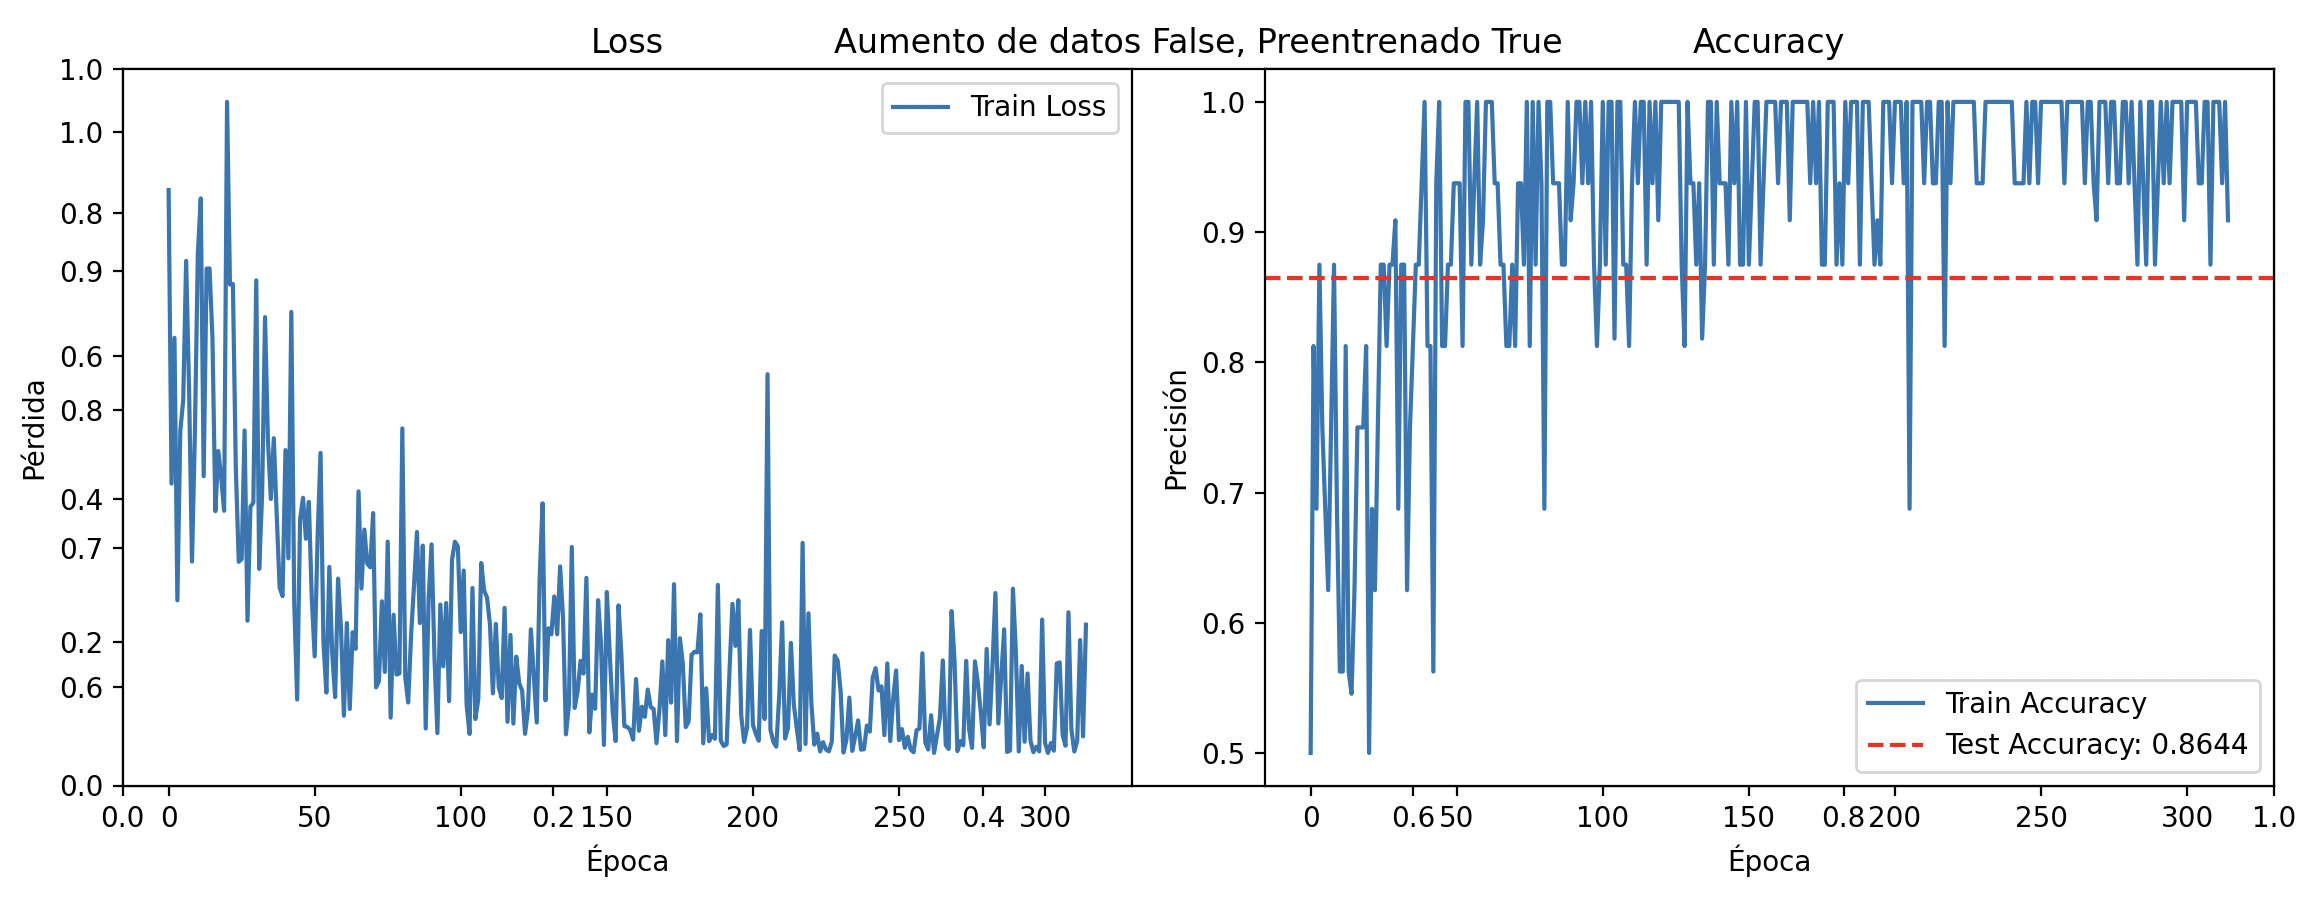
\includegraphics[width=0.9\linewidth]{lossEj2}
	\label{fig:lossEj2}
	\caption{Loss y Accuracy para el segundo ejercicio}
\end{figure}

\begin{figure}[h]
	\centering
	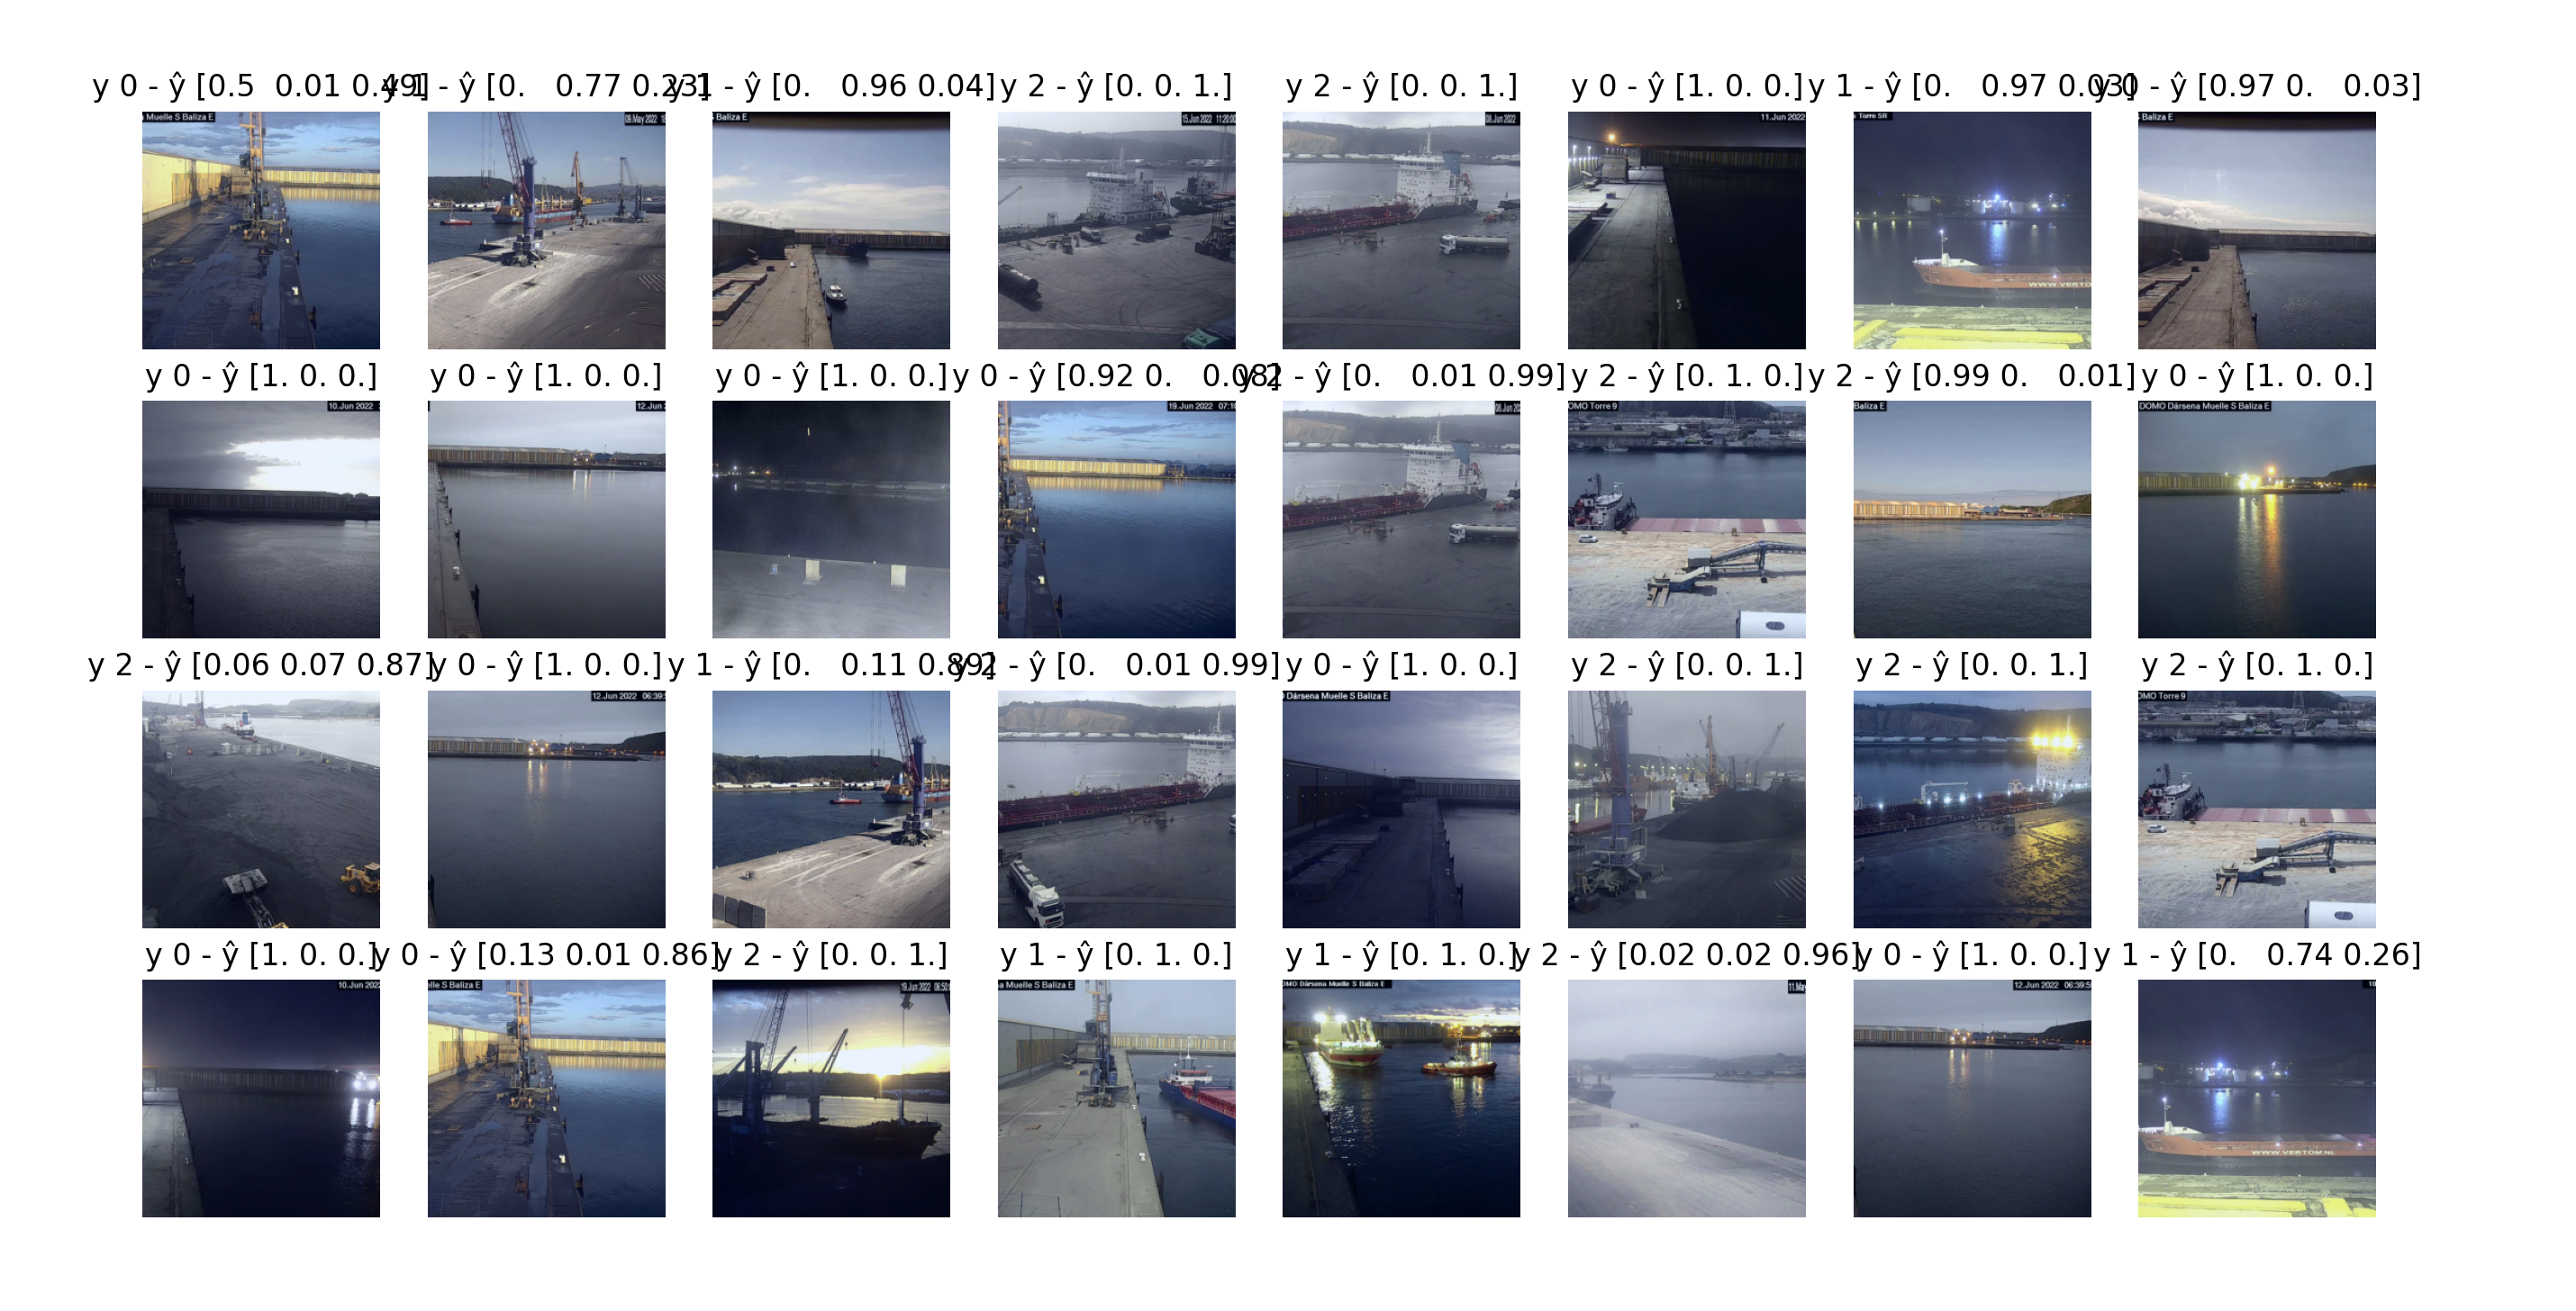
\includegraphics[width=0.8\linewidth]{imagenesEj2}
	\label{fig:imagenesEj2}
	\caption{Imágenes con su etiqueta correcta y el vector SoftMax predicha por la red para el segundo ejercicio}
\end{figure}


\section*{Options}

\begin{itemize}
    \item \texttt{-h, --help} \hfill Show this help message and exit
    \item \texttt{--root\_dir ROOT\_DIR} \hfill Root directory containing the image folders
    \item \texttt{--data\_augmentation} \hfill Apply data augmentation and include cropped ship images
    \item \texttt{--docked} \hfill Include docked status in labels
    \item \texttt{--not\_train} \hfill Not train the model, used in conjunction with \texttt{--test\_images}
    \item \texttt{--train\_ratio TRAIN\_RATIO} \hfill Ratio of training data to total data
    \item \texttt{--unbalanced} \hfill Unless specified, class balancing will be applied
    \item \texttt{--pretrained} \hfill Use pretrained weights for the model
    \item \texttt{--mlp\_head} \hfill Use a 2-layer MLP in the head of the model
    \item \texttt{--model\_path MODEL\_PATH} \hfill Path to save or load the model
    \item \texttt{--load\_model} \hfill Load a pretrained model instead of training
    \item \texttt{--arquitecture ARQUITECTURE} \hfill Model architecture, default is \texttt{efficientnet\_b4}.
    \item \texttt{--batch\_size BATCH\_SIZE} \hfill Batch size for training and testing
    \item \texttt{--num\_workers NUM\_WORKERS} \hfill Number of workers for data loading
    \item \texttt{--num\_epochs NUM\_EPOCHS} \hfill Number of epochs for training
    \item \texttt{--patience PATIENCE} \hfill Patience for early stopping
    \item \texttt{--lr\_patience LR\_PATIENCE} \hfill Patience for reducing learning rate
    \item \texttt{--learning\_rate LEARNING\_RATE} \hfill Learning rate for optimizer
    \item \texttt{--l2\_lambda L2\_LAMBDA} \hfill Lambda for L2 weight decay regularization
    \item \texttt{--show} \hfill Show figures instead of saving them
    \item \texttt{--device DEVICE} \hfill Device, default is \texttt{mps}
    \item \texttt{--test\_images TEST\_IMAGES [TEST\_IMAGES ...]} \hfill List of image paths to test individually
\end{itemize}








\newpage

\bibliographystyle{plain}
\bibliography{referencias}



\end{document}

